\documentclass[pdftex,12pt,a4paper]{article}

\usepackage{graphicx}  
\usepackage[margin=2.5cm]{geometry}
\usepackage{breakcites}
\usepackage{indentfirst}
\usepackage{pgfgantt}
\usepackage{pdflscape}
\usepackage{float}
\usepackage{epsfig}
\usepackage{epstopdf}
\usepackage[cmex10]{amsmath}
\usepackage{stfloats}
\usepackage{multirow}

\renewcommand{\refname}{REFERENCES}
\linespread{1.3}

\usepackage{mathtools}
%\newcommand{\HRule}{\rule{\linewidth}{0.5mm}}
\thispagestyle{empty}
\begin{document}
\begin{titlepage}
\begin{center}
\textbf{}\\
\textbf{\Large{ISTANBUL TECHNICAL UNIVERSITY}}\\
\vspace{0.5cm}
\textbf{\Large{COMPUTER ENGINEERING DEPARTMENT}}\\
\vspace{2cm}
\textbf{\Large{BLG 222E\\ Computer Organization \\ Project 1}}\\
\vspace{2.8cm}
\begin{table}[ht]
\centering
\Large{
\begin{tabular}{lcl}
\textbf{PROJECT DATE}  & : & 24.05.2023\\
\end{tabular}}
\end{table}
\vspace{1cm}
\textbf{\Large{GROUP MEMBERS:}}\\
\begin{table}[ht]
\centering
\Large{
\begin{tabular}{rcl}
150220762  & : & Muhammed Yusuf Mermer (Group Representative)  \\
150210071  & : & Emre Çamlıca \\
150200091  & : & Hakan Duran \\
\end{tabular}}
\end{table}
\vspace{2.8cm}
\textbf{\Large{SPRING 2023}}

\end{center}

\end{titlepage}

\thispagestyle{empty}
\addtocontents{toc}{\contentsline {section}{\numberline {}FRONT COVER}{}}
\addtocontents{toc}{\contentsline {section}{\numberline {}CONTENTS}{}}
\setcounter{tocdepth}{4}
\tableofcontents
\clearpage

\setcounter{page}{1}
\section{INTRODUCTION}
In this project our purpose was to design a hardwired control unit. To achive 
this we firstly implemented small components of this system. Yusuf did the fetch and decode parts, Hakan did the instructions without memory reference and Emre did the instructions with memory reference. Yusuf also wrote the test bench and tested the system with Hakan.

At first, Yusuf has designed the fetch cycle. Then Hakan and Emre designed the execute part. Hakan and Yusuf then tested the project and corrected the errors.


\section{IMPLEMENTATIONS AND EXPLANATIONS }
\subsection{Fetch Cycle, Counter and Decoding}
In our implementations, we made only counter module seperated from the 
combined system. It could have also been designed inside of overall 
combined system as a register, but this was our design choice. It takes 
clock as input, because at every positive edge we increase our timing signal
by 1. However, to prevent unexpected result in the current postive edge we wait for
0.25 ns in our implementation.

Not only clock, but also reset signal taken as input for this module
to return inital value for the timing signal. When it reset, it returns value 4 bit
binary 1111 which is equal to -0001, this is been made because reset signal 
does not depend on clock; therofore, after the reset we wait for new clock signal 
to start new operations. New operations will be started with timing signal 0.

INtial ve ilk always blcoklarından bahset**********************************

For our combined module, we have  after making all necesessary connections, 

When timing signal 0 arrives to our combined system, it starts to fetch cycle. Our 
fetch cycle is totally takes 3 cycles. It has been made 3 cycles to prvent 
changes unintended changes on the PC and IR.

At first (0th) cycle of the fetch, we made 





\subsection{Instructions With Address Reference}

\subsection{Instructions Without Address Reference}






\section{OVERALL DESIGN PHOTO}


\begin{figure}[H]
    \centering
    \includegraphics[width=1\textwidth]{photos/design.png}	
    \caption{overall design photo}
    \label{implementation}
\end{figure}








\section{SIMULATION RESULTS}


\begin{figure}[H]
    \centering
    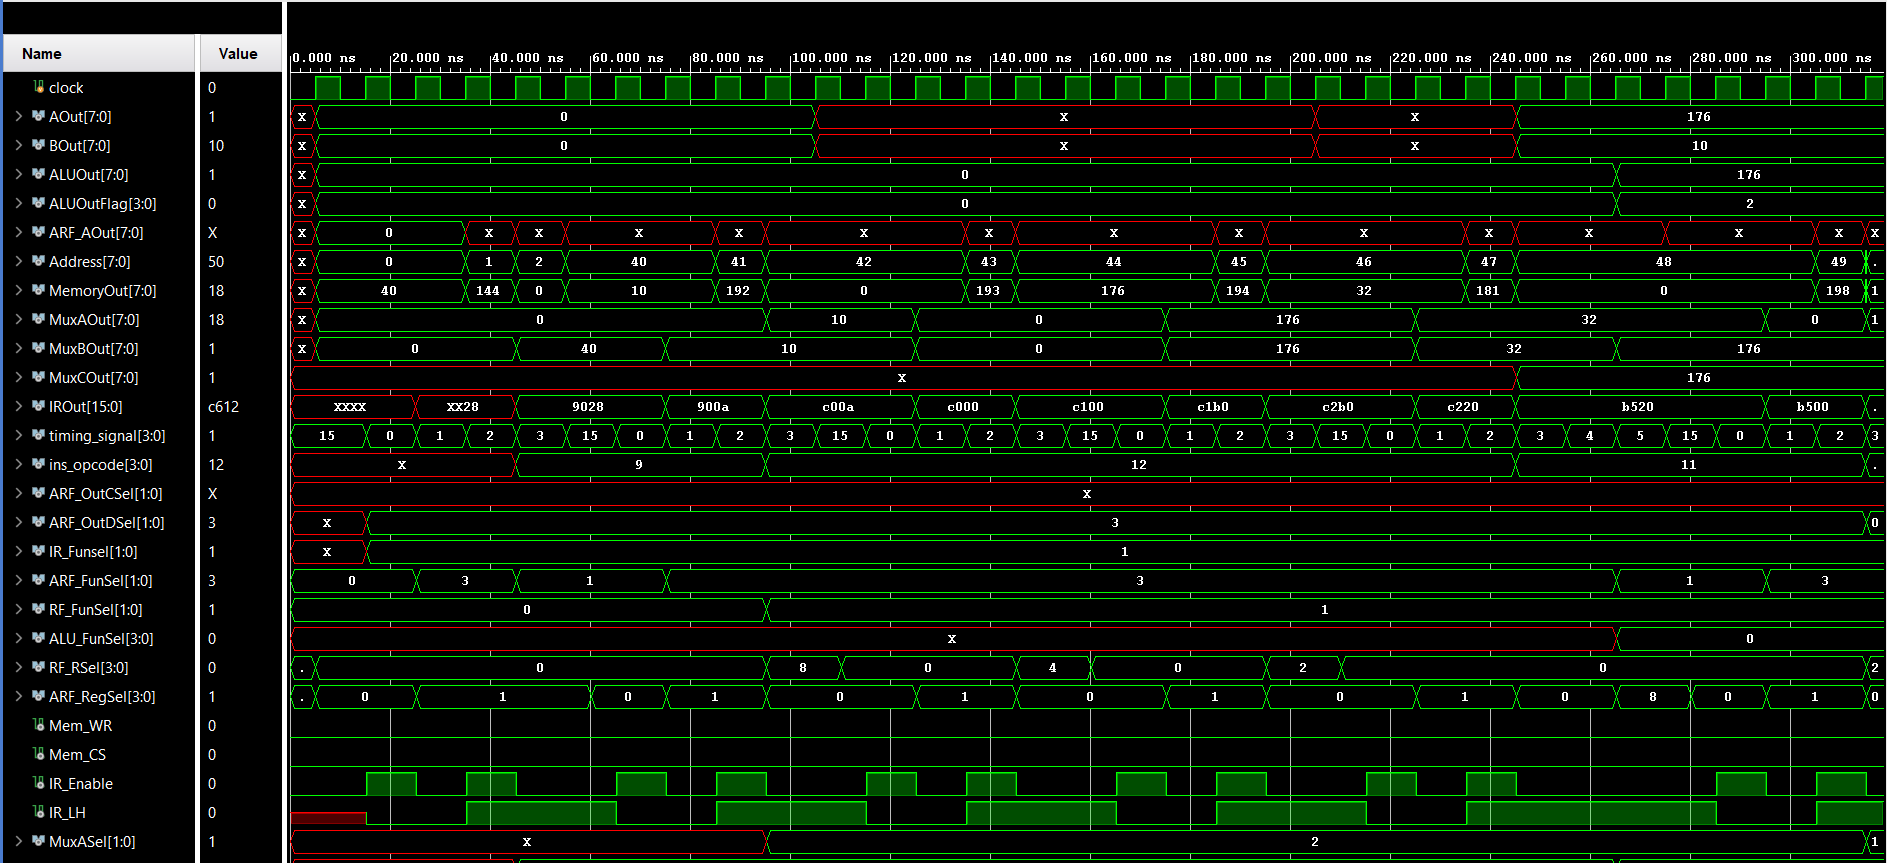
\includegraphics[width=1\textwidth]{photos/system_result_1.png}	
    \caption{simulation of system}
    \label{implementation}
\end{figure}


\begin{figure}[H]
    \centering
    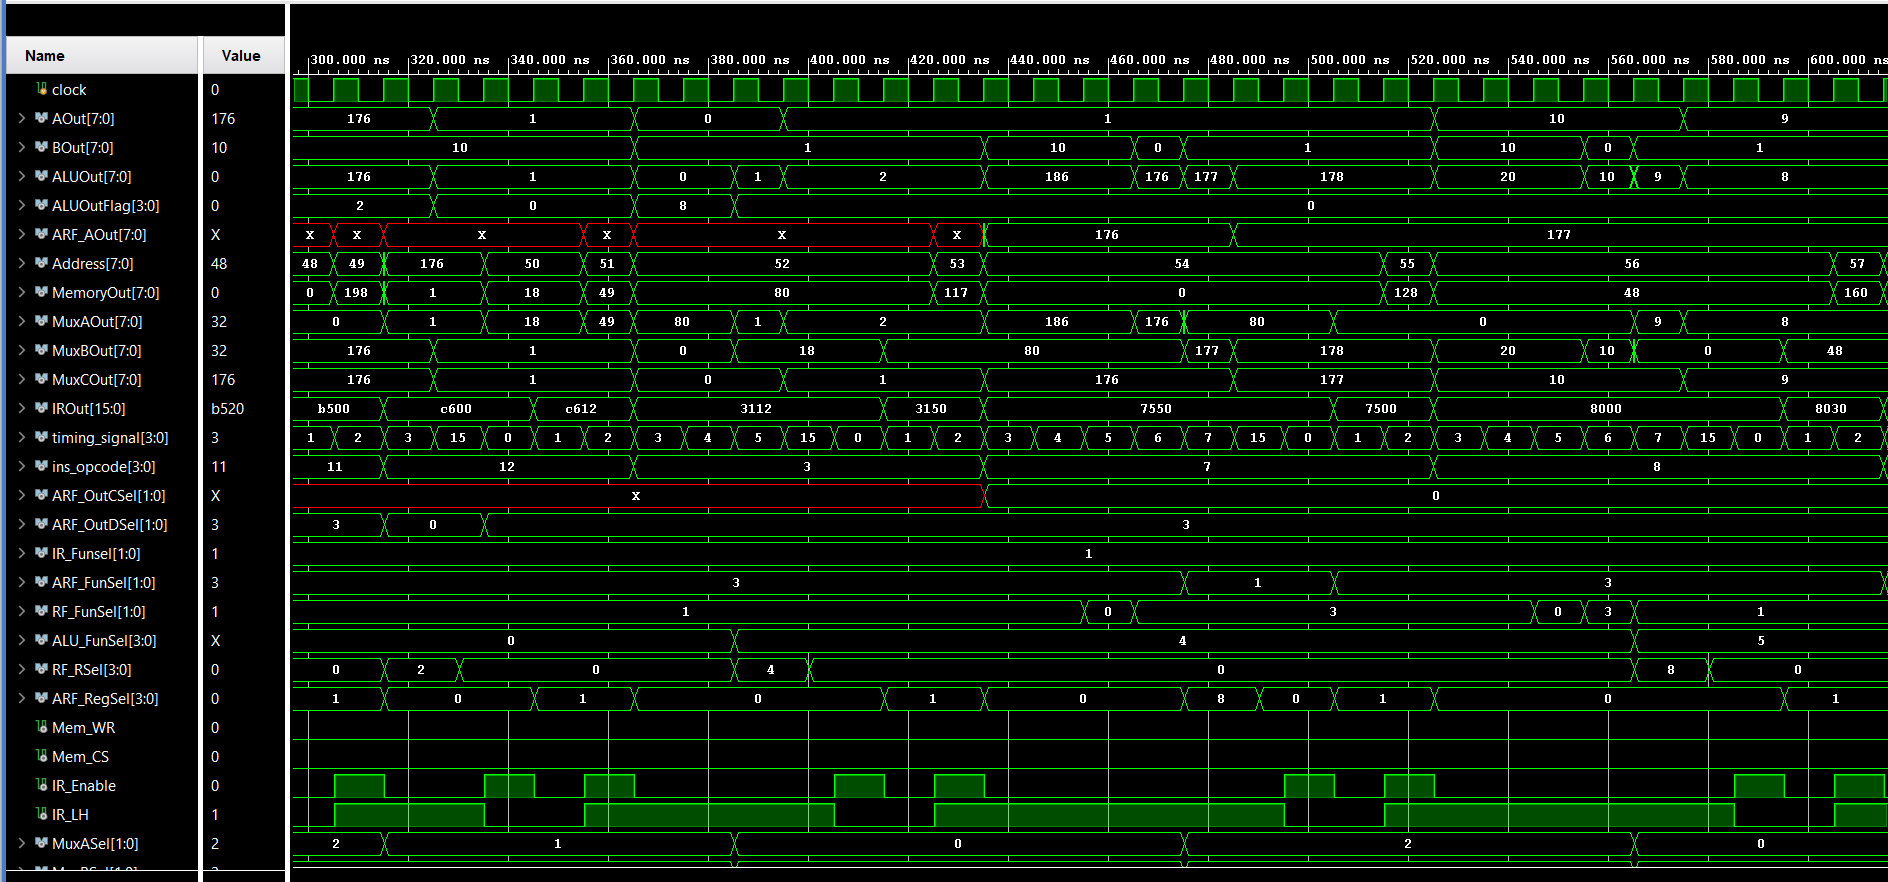
\includegraphics[width=1\textwidth]{photos/system_result_2.png}	
    \caption{simulation of system}
    \label{implementation}
\end{figure}


\begin{figure}[H]
    \centering
    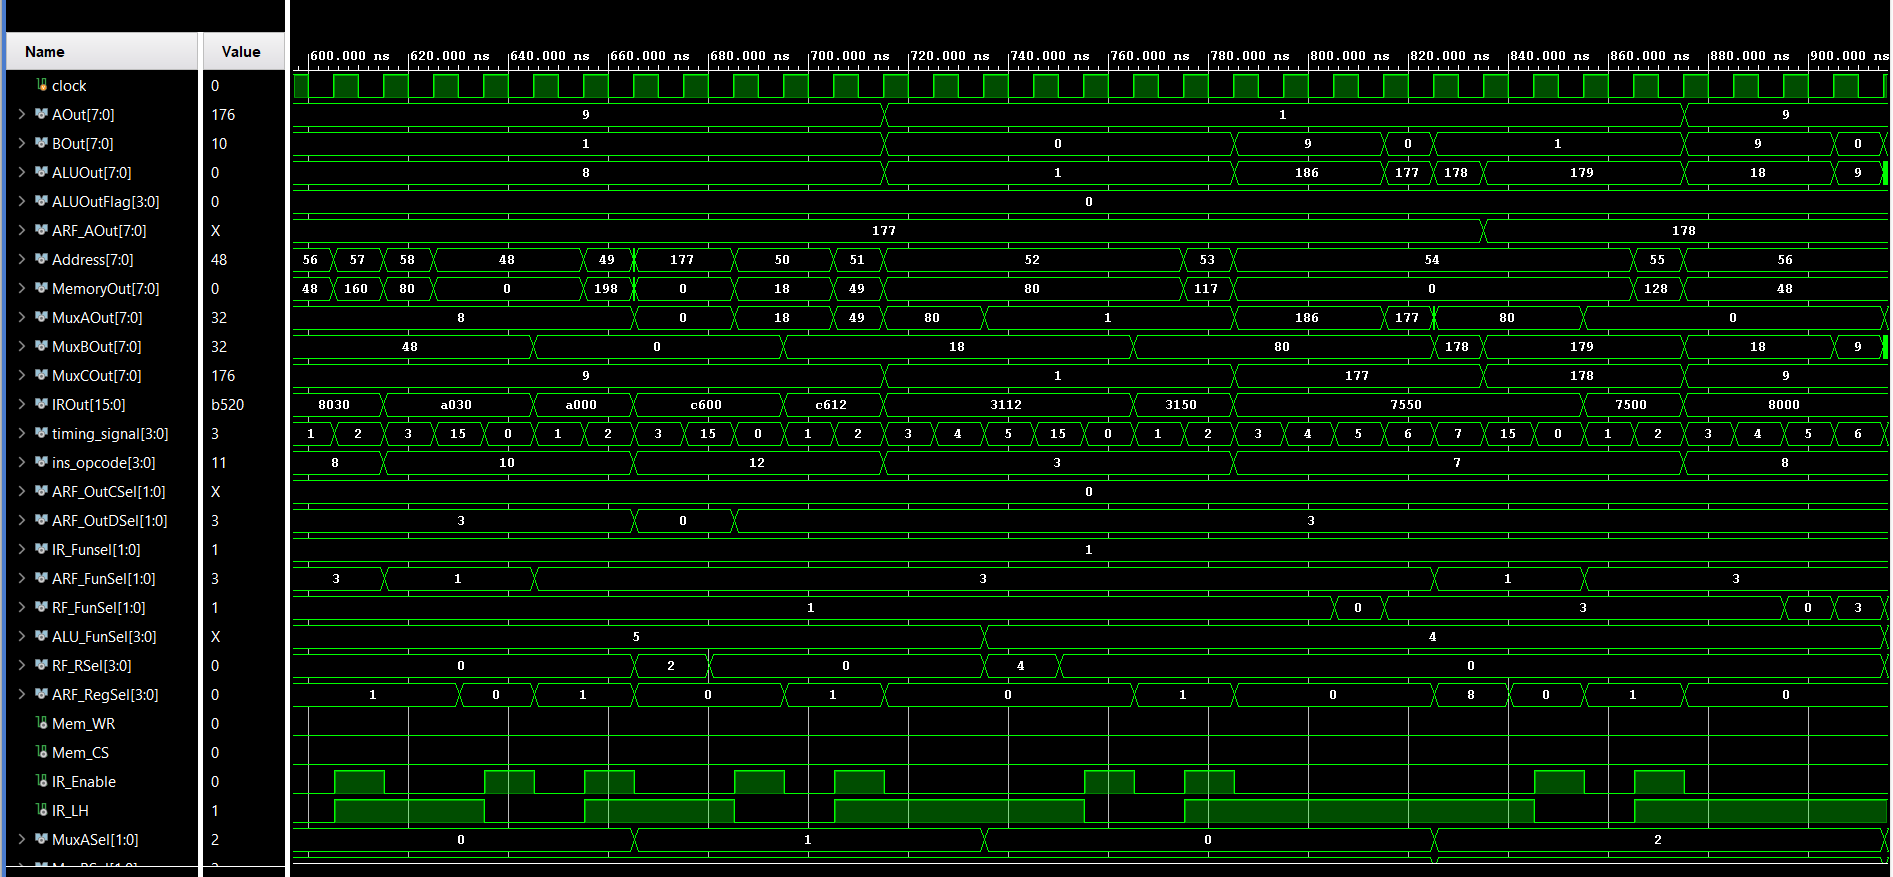
\includegraphics[width=1\textwidth]{photos/system_result_3.png}	
    \caption{simulation of system}
    \label{implementation}
\end{figure}



\begin{figure}[H]
    \centering
    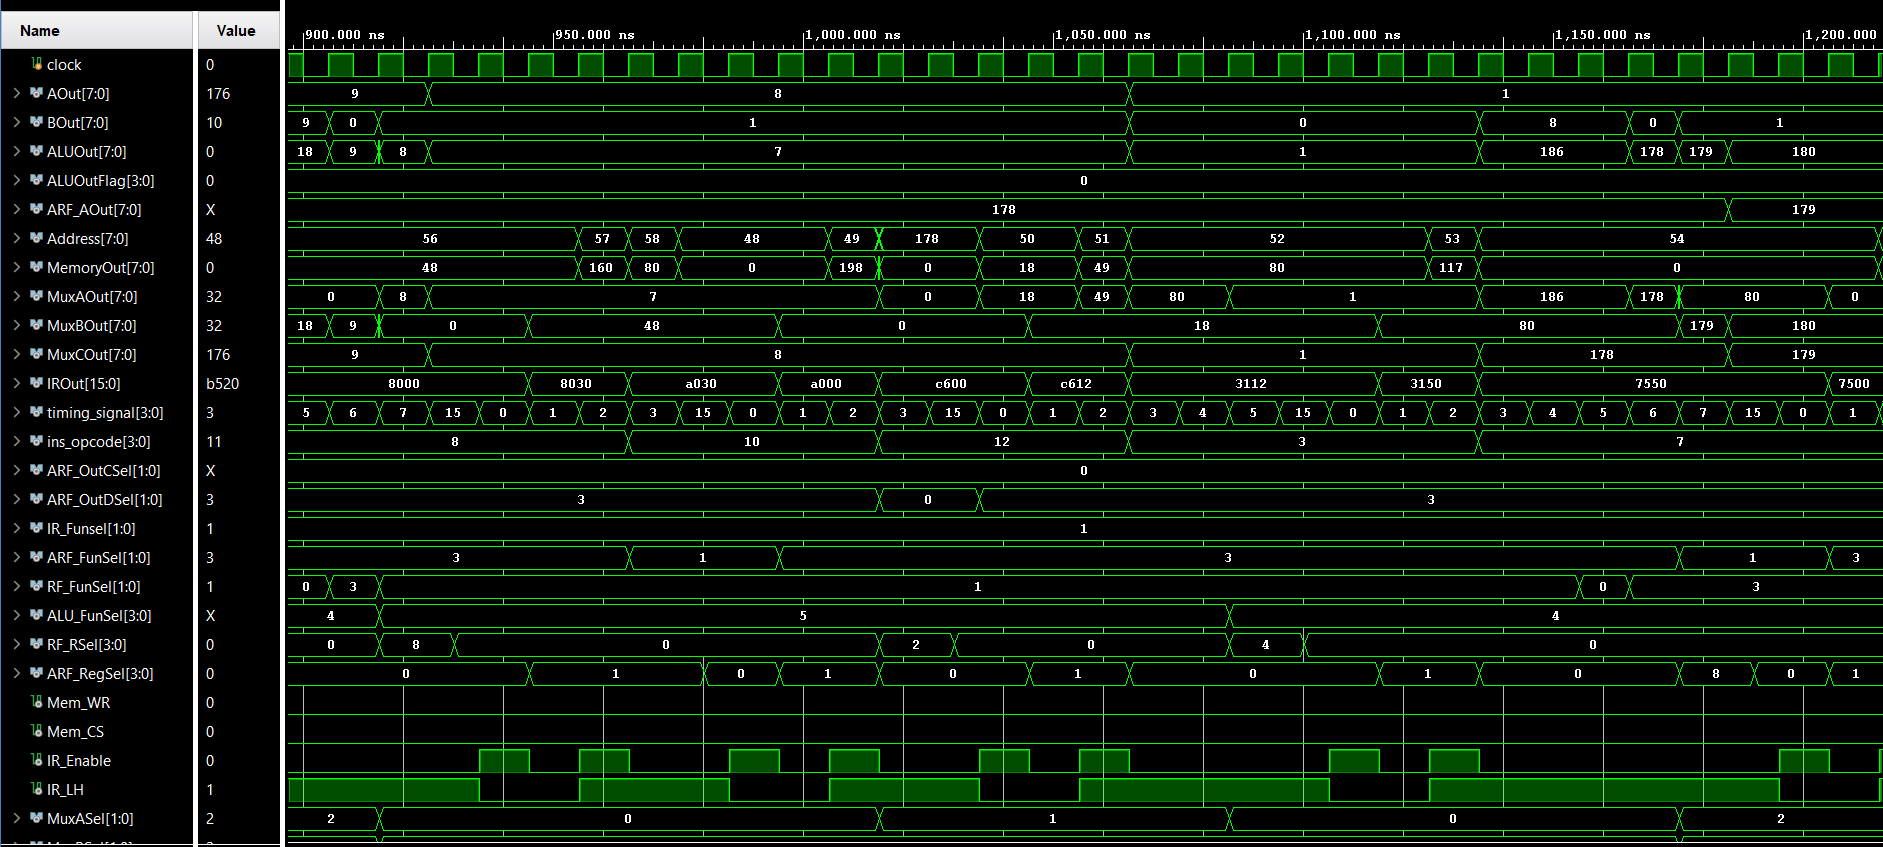
\includegraphics[width=1\textwidth]{photos/system_result_4.png}	
    \caption{simulation of system}
    \label{implementation}
\end{figure}

\begin{figure}[H]
    \centering
    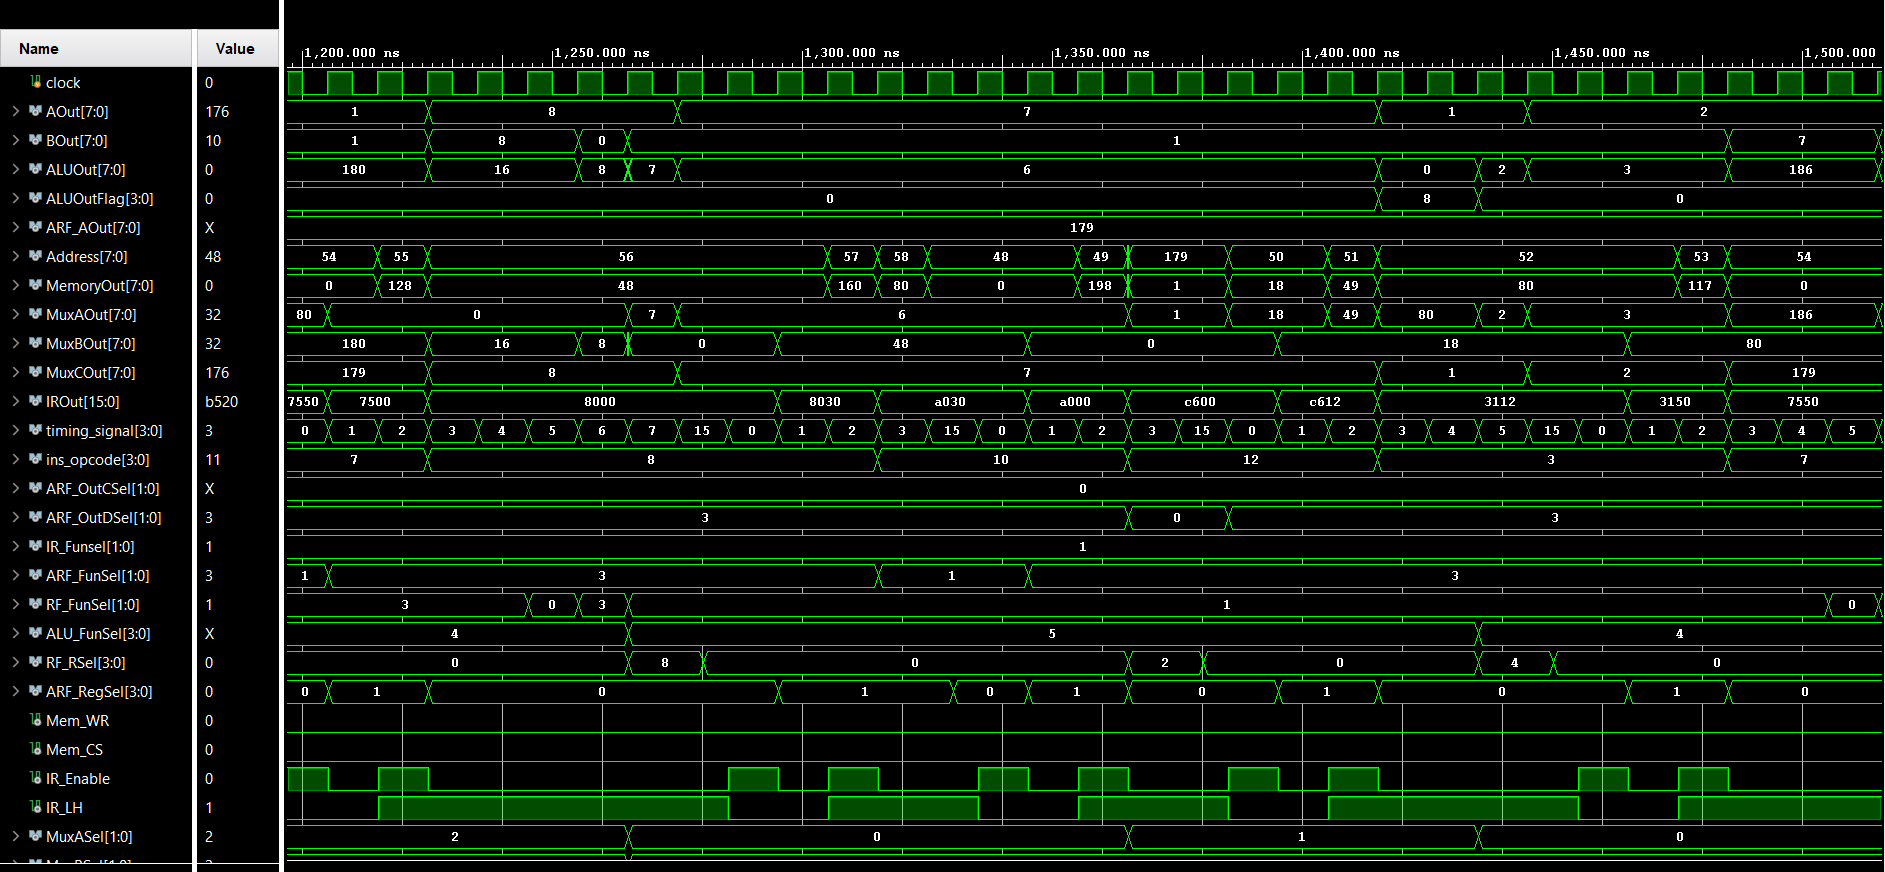
\includegraphics[width=1\textwidth]{photos/system_result_5.png}	
    \caption{simulation of system}
    \label{implementation}
\end{figure}


\begin{figure}[H]
    \centering
    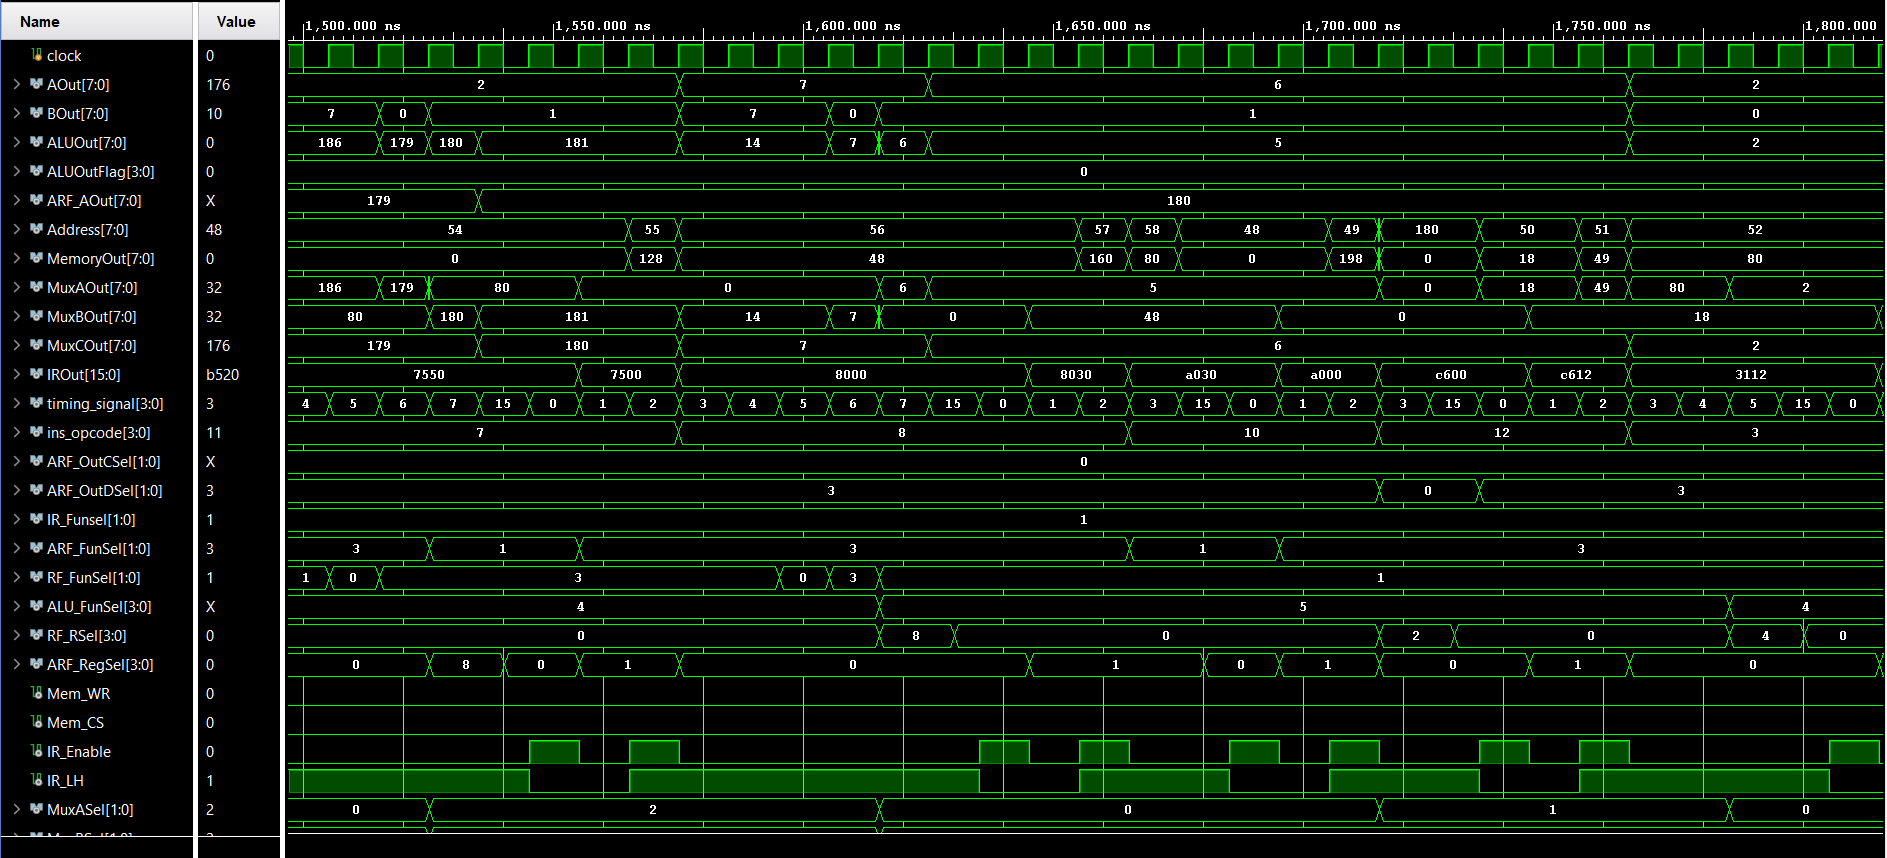
\includegraphics[width=1\textwidth]{photos/system_result_6.png}	
    \caption{simulation of system}
    \label{implementation}
\end{figure}


\begin{figure}[H]
    \centering
    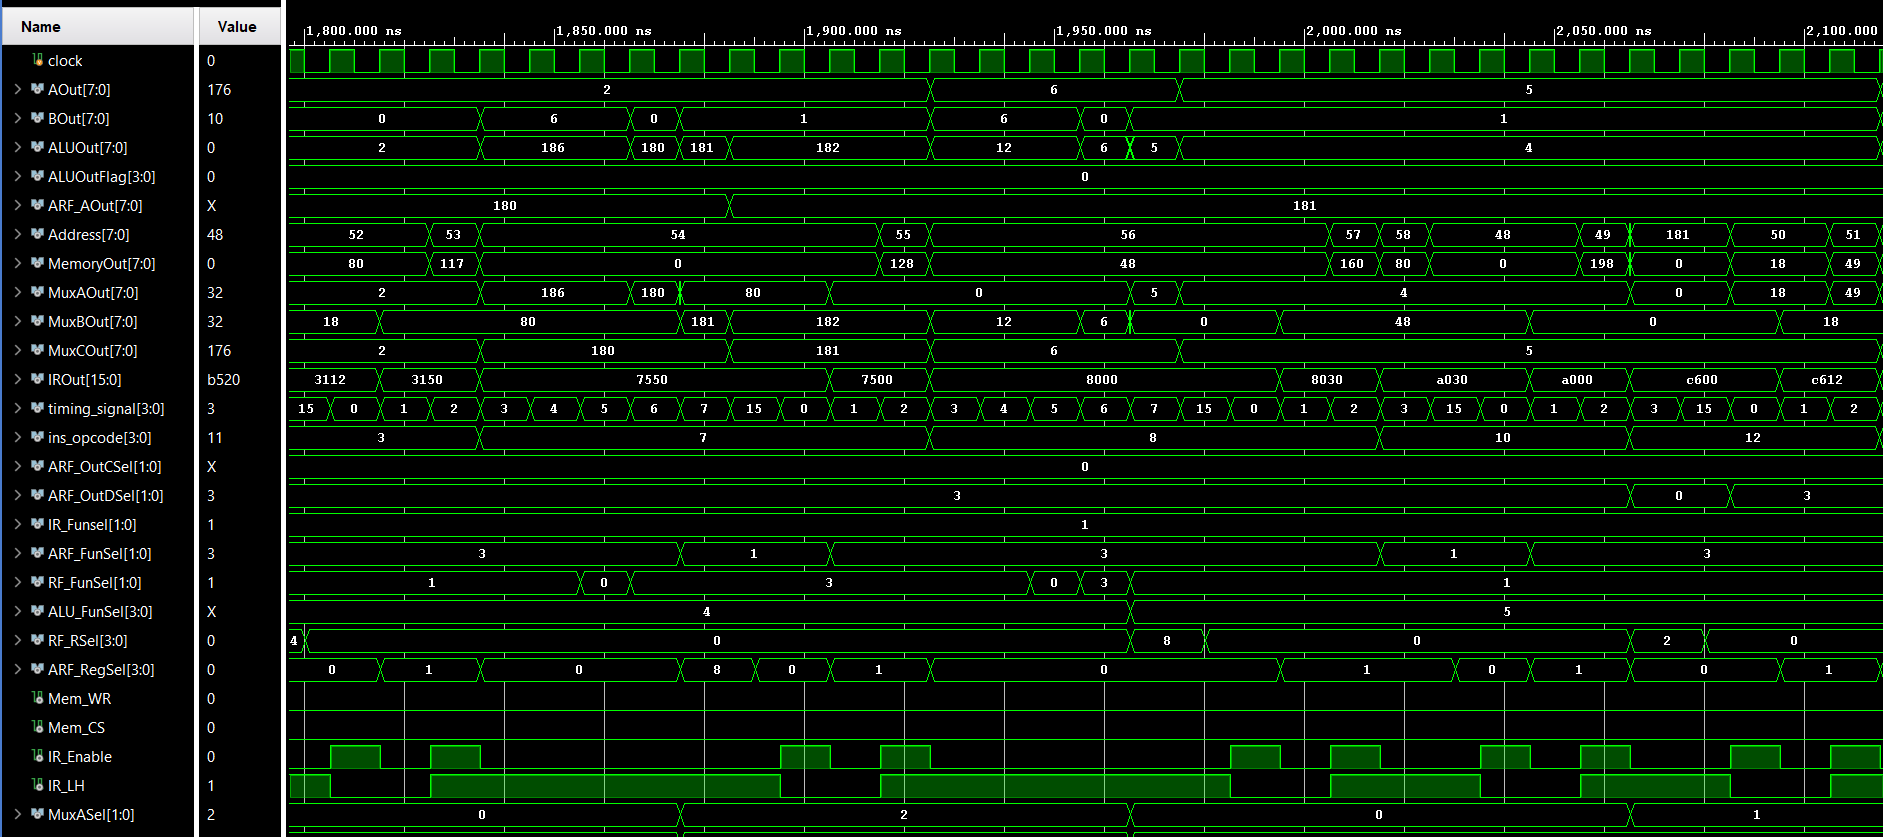
\includegraphics[width=1\textwidth]{photos/system_result_7.png}	
    \caption{simulation of system}
    \label{implementation}
\end{figure}

\begin{figure}[H]
    \centering
    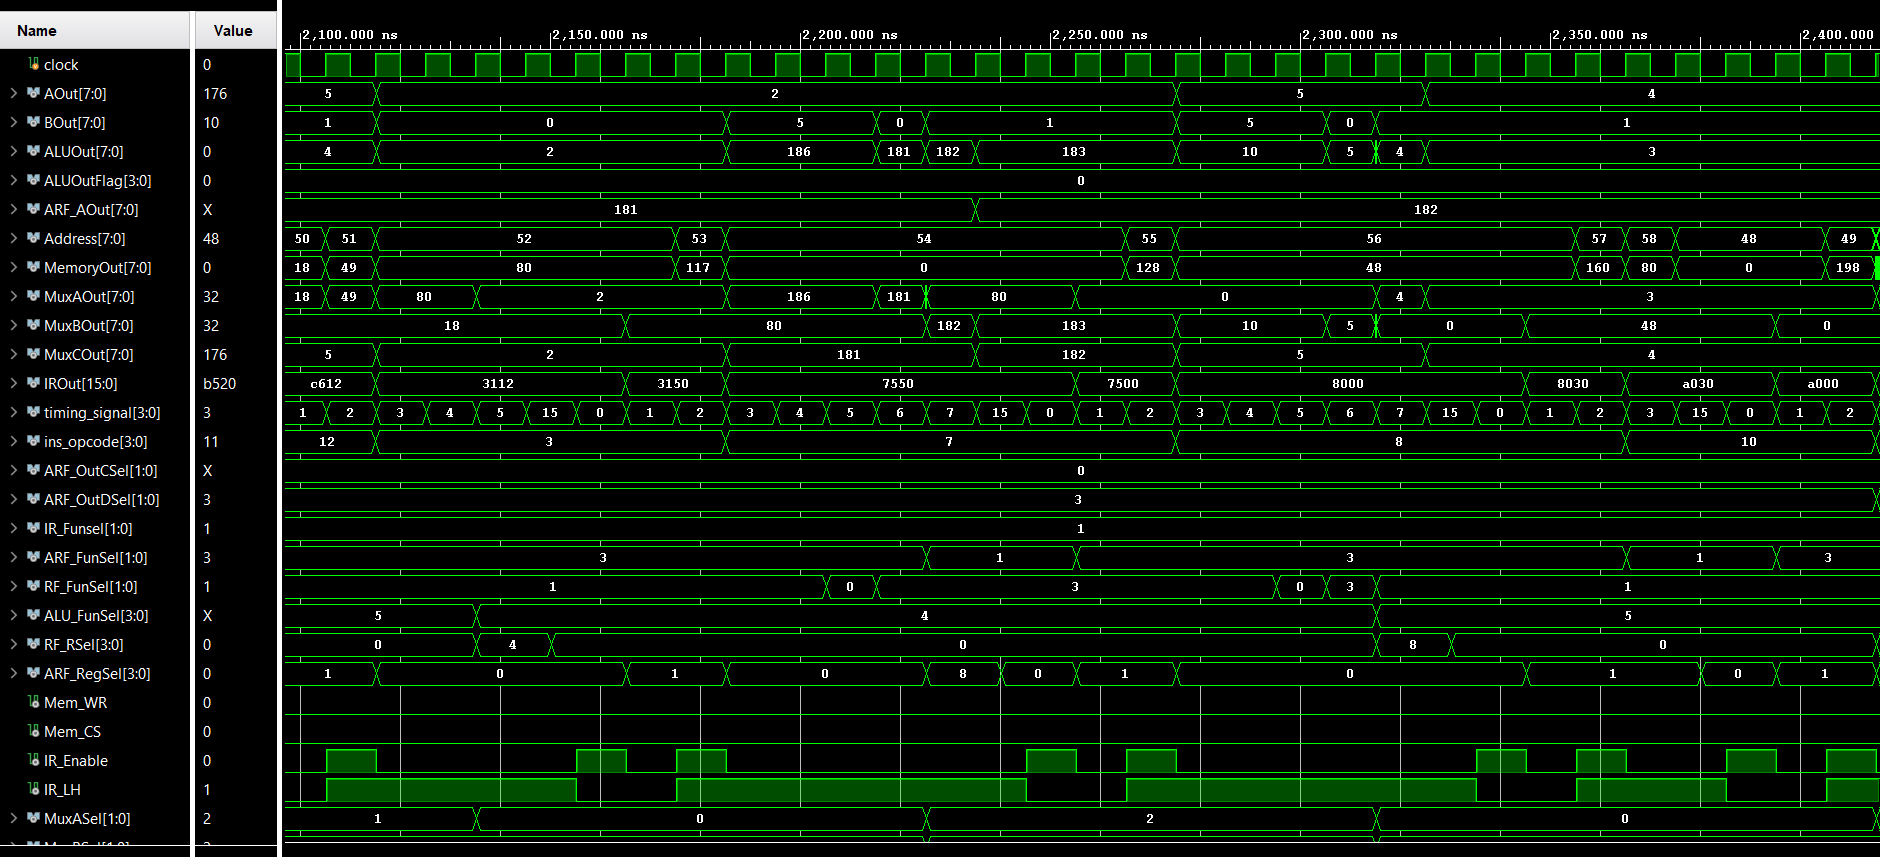
\includegraphics[width=1\textwidth]{photos/system_result_8.png}	
    \caption{simulation of system}
    \label{implementation}
\end{figure}

\begin{figure}[H]
    \centering
    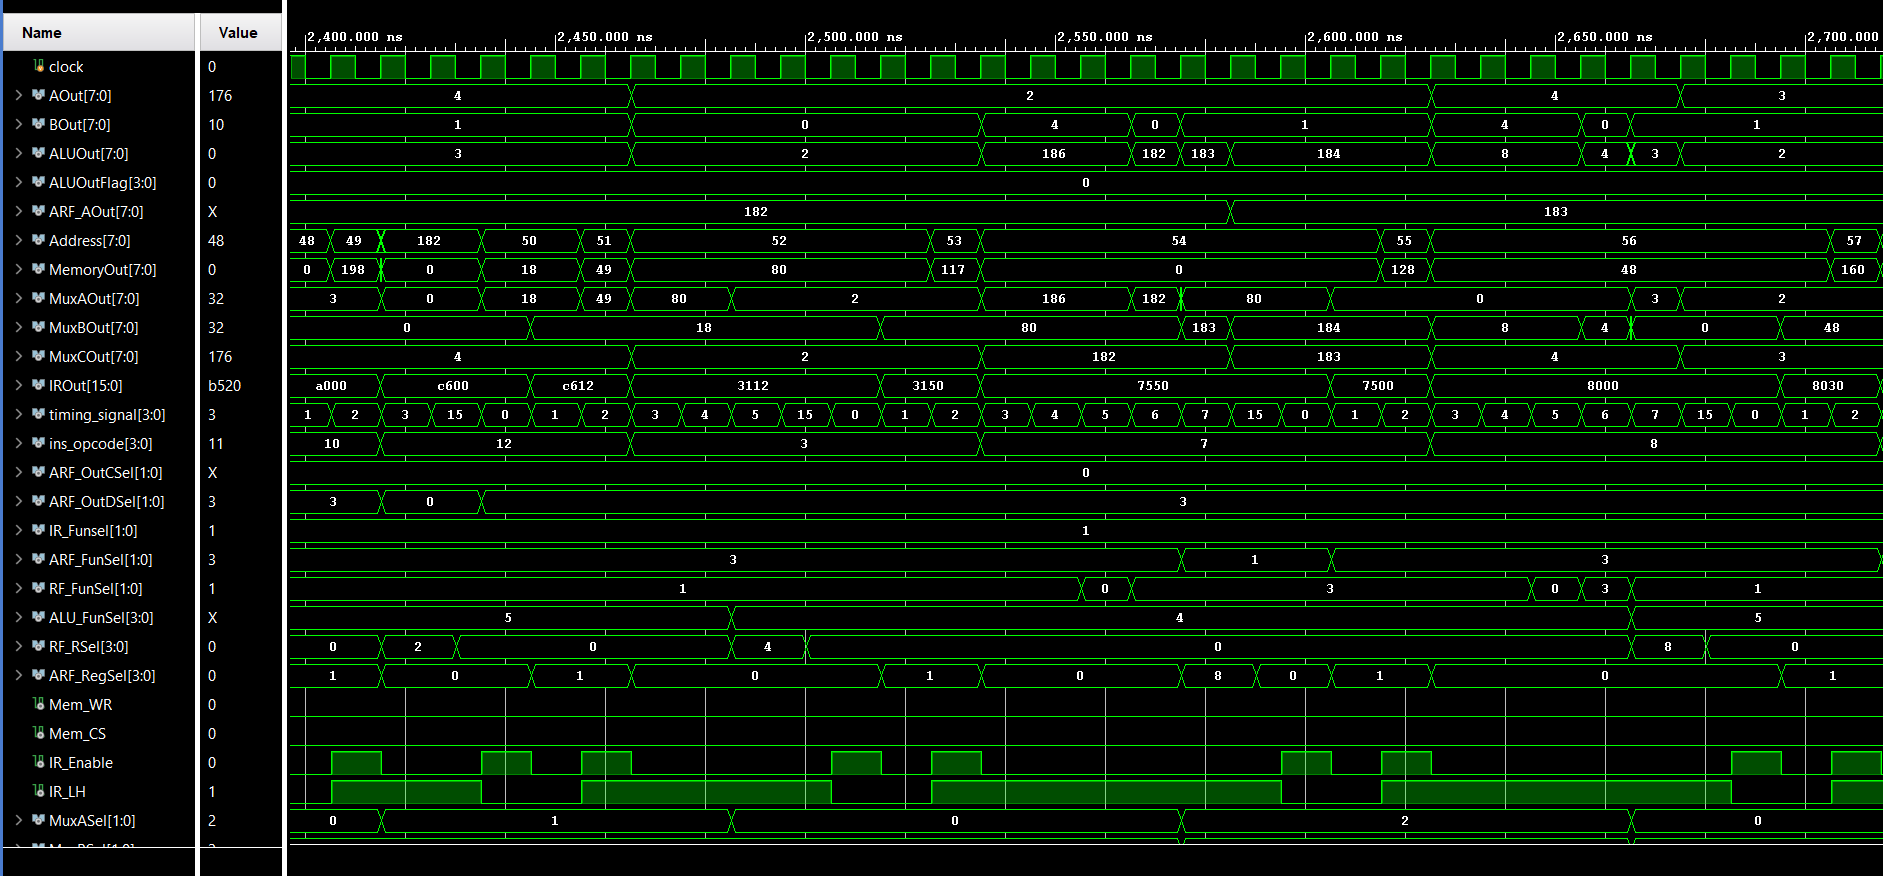
\includegraphics[width=1\textwidth]{photos/system_result_9.png}	
    \caption{simulation of system}
    \label{implementation}
\end{figure}

\begin{figure}[H]
    \centering
    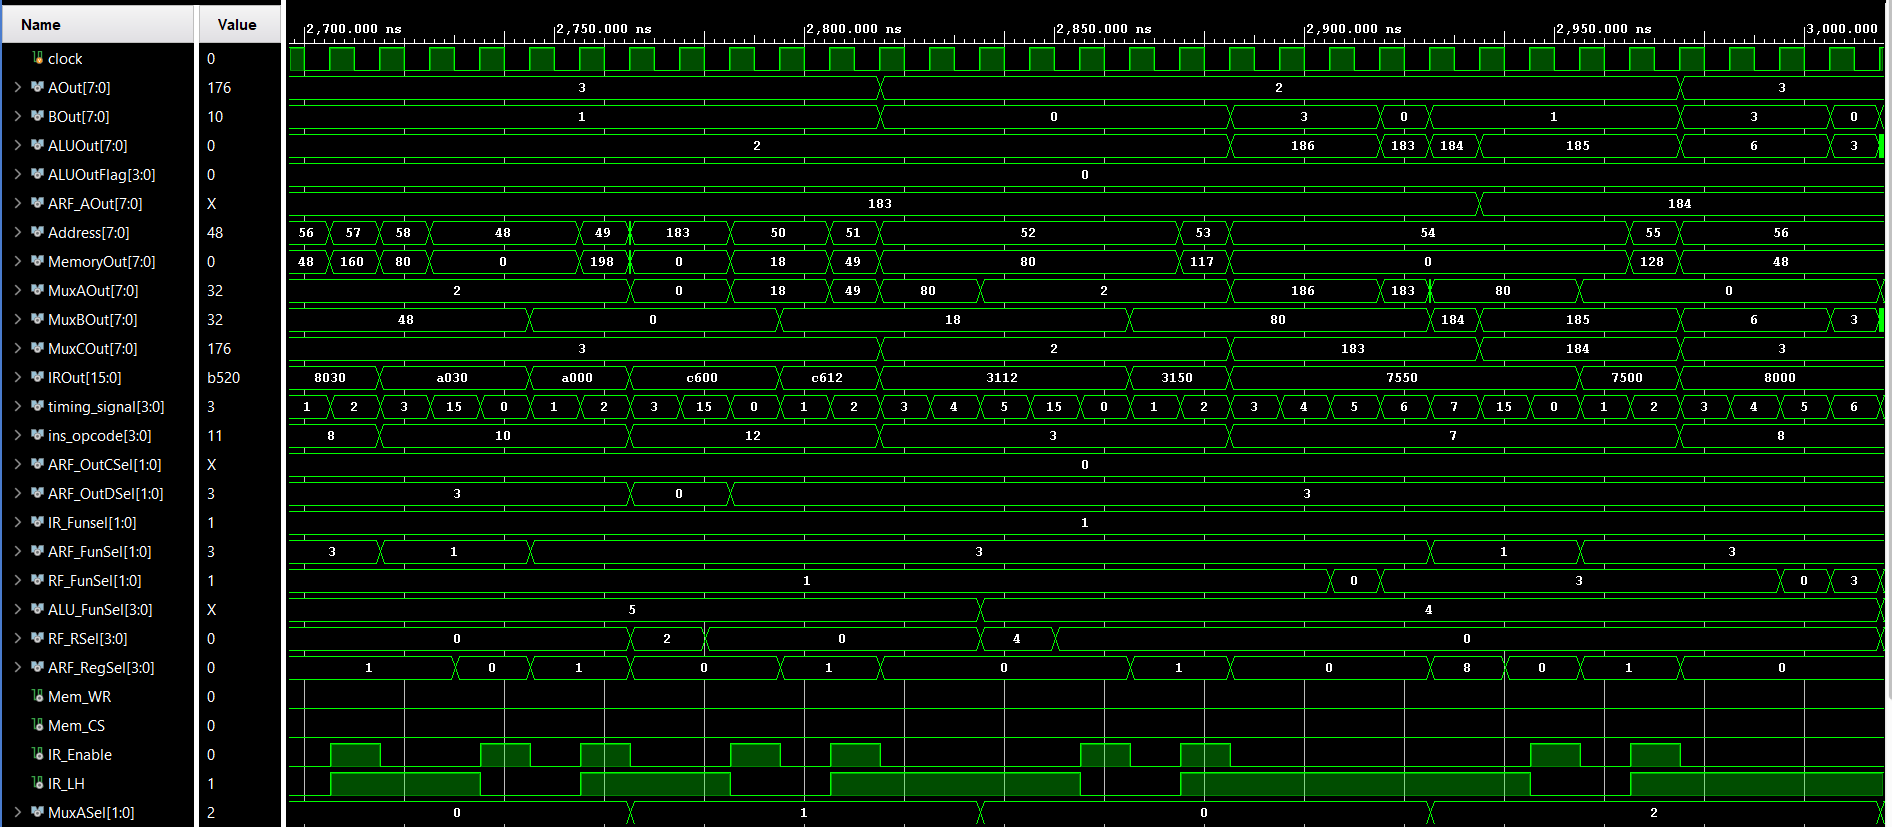
\includegraphics[width=1\textwidth]{photos/system_result_10.png}	
    \caption{simulation of system}
    \label{implementation}
\end{figure}

\begin{figure}[H]
    \centering
    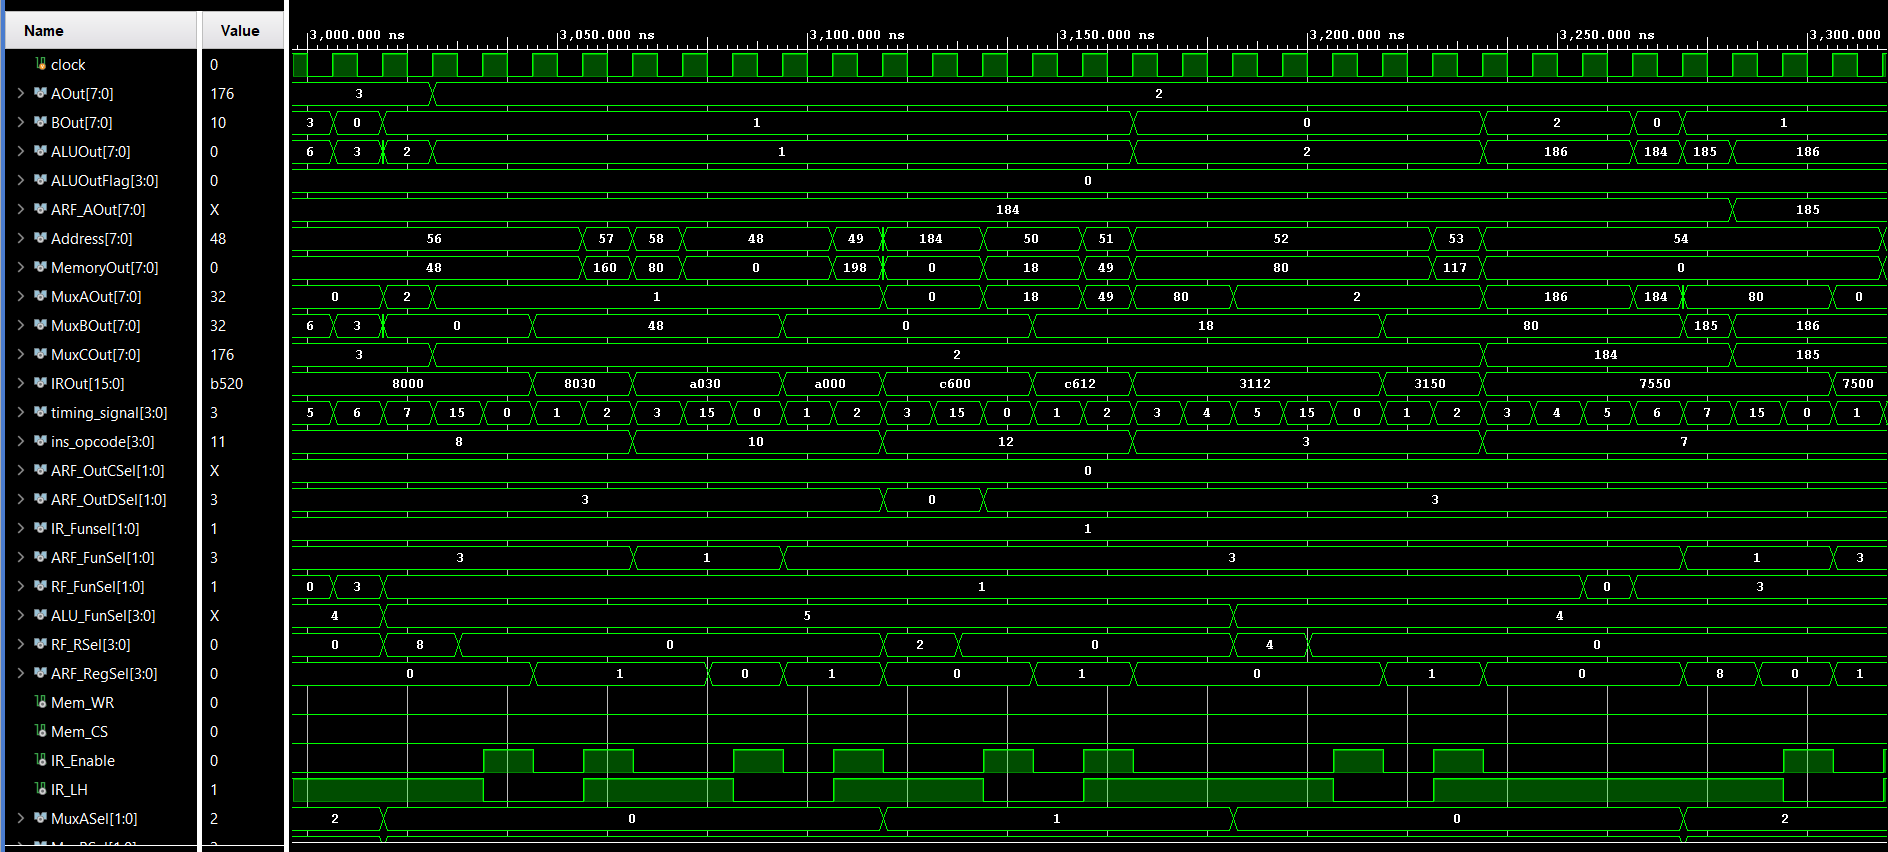
\includegraphics[width=1\textwidth]{photos/system_result_11.png}	
    \caption{simulation of system}
    \label{implementation}
\end{figure}

\begin{figure}[H]
    \centering
    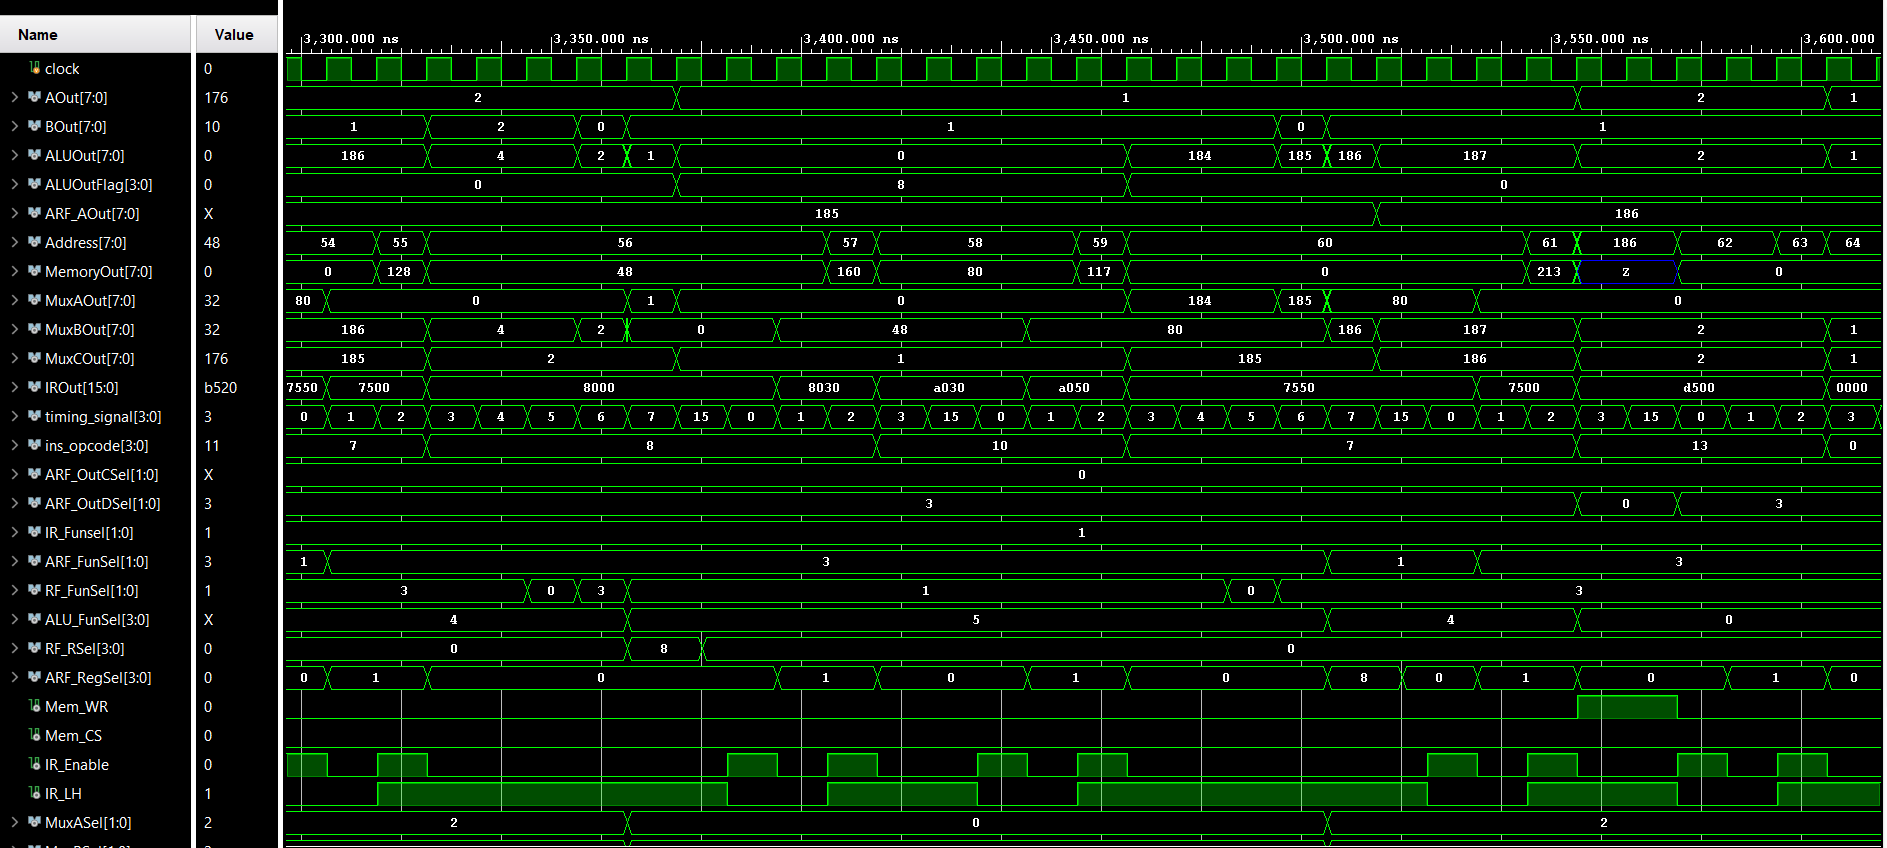
\includegraphics[width=1\textwidth]{photos/system_result_12.png}	
    \caption{simulation of system}
    \label{implementation}
\end{figure}

\begin{figure}[H]
    \centering
    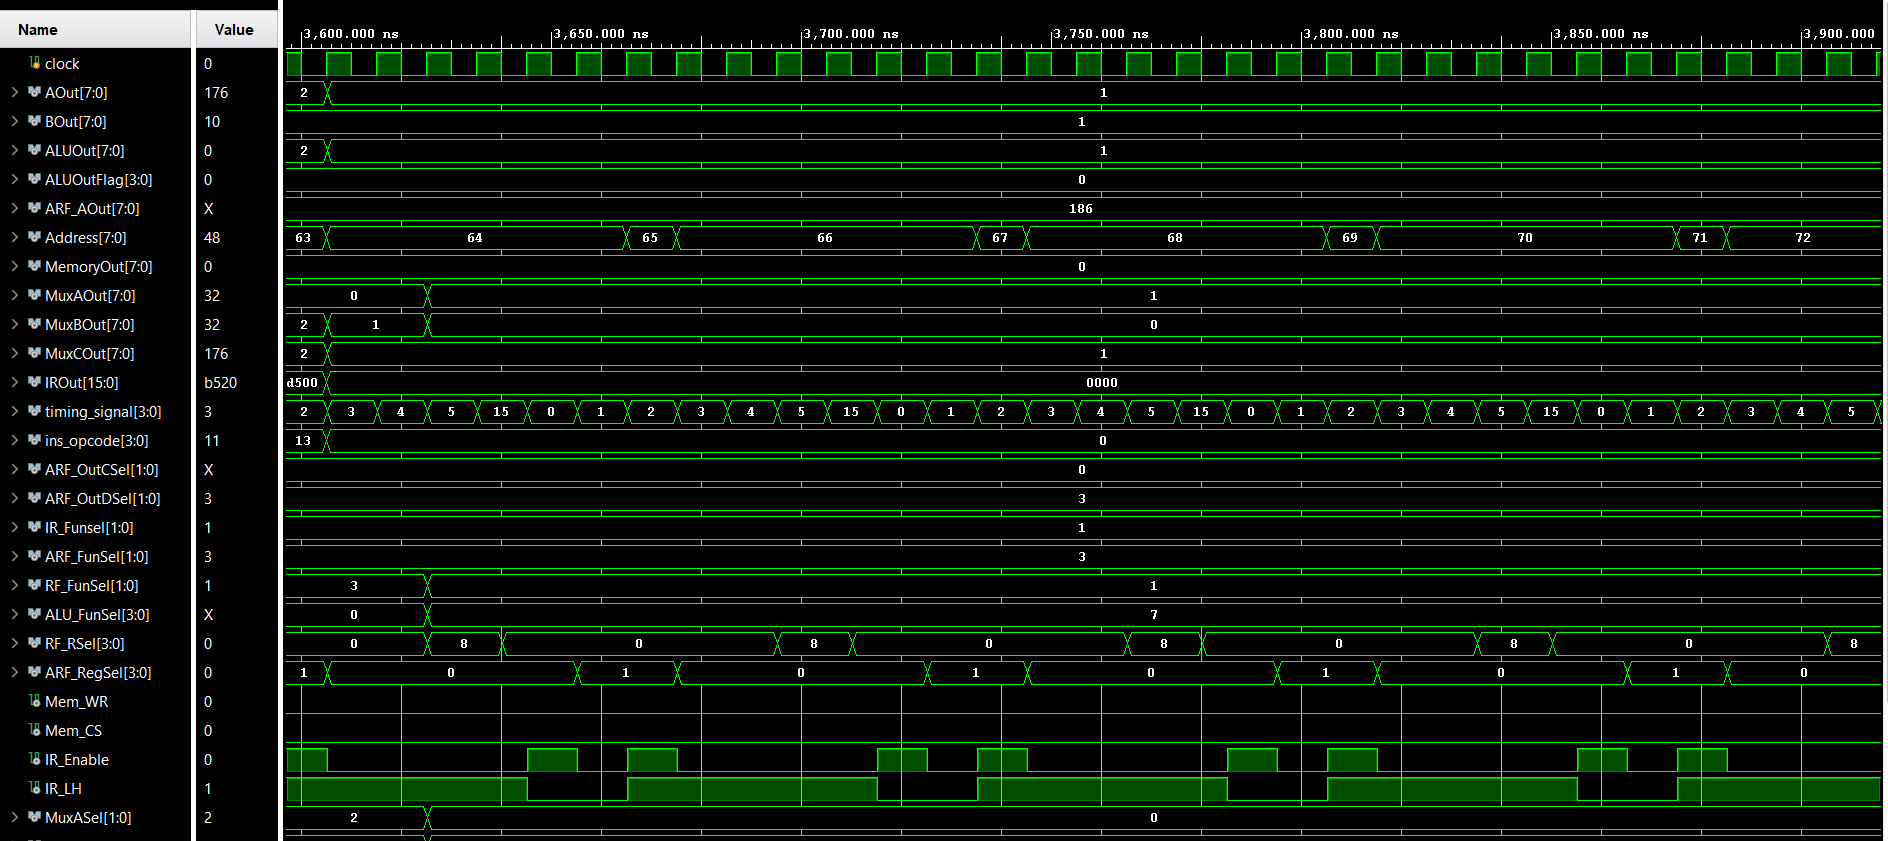
\includegraphics[width=1\textwidth]{photos/system_result_13.png}	
    \caption{simulation of system}
    \label{implementation}
\end{figure}




\section{DISCUSSION}

ilk önce nasıl fetch cycle yaptığından bahset. 




\section{CONCLUSION}
In this project we designed a hardwired control unit with the help of the ones we created in the first project. 

\end{document}